\chapter{В каких населённых пунктах России больше рождаётся учёных, в сельских или городских?}
\label{ch:human-settlement}

В главе исследуется объект Викиданных \wdqName{населённый пункт}{486972} и его свойства. 
В каждом из разделов представлены задачи, решённые с помощью SPARQL-запросов. 
%
%%%%%%%%%%%%%%%% Упражнение 1 %%%%%%%%%%%%%%%% 
\marginnote{Подсчитайте, сколько человек на км\textsuperscript{2} живёт в \ruwiki{4dNv}{Барабинске} 
и в~\ruwiki{4dNt}{Алейске}? В каком из этих \emph{населённых пунктов} плотность населения выше?

См. ответ~\ref{answer:human_settlements_density} на с.~\pageref{answer:human_settlements_density}.%
}

Был получен список населённых пунктов, 
построены пузырьковые диаграммы с количеством населения в <<населённых пунктах>> по странам. 
Построена диаграмма, показывающая долю населения, 
проживающего в населённых пунктах относительно всего населения страны. 
Диаграмма показала, что высокий процент населения, проживающего в населённых пунктах, 
приходится на сельскохозяйственные страны, в то время как в более индустриальных странах 
меньшая доля населения проживает в населённых пунктах. 

На 2017 год Википедия описывала примерно половину населённых пунктов (75 тыс.), 
Викиданные содержали менее 3\% таких поселений (4 тыс.) относительно данных переписи за 2010 год (155,5 тыс.). 
На 2021 год Викиданные содержат менее 12\% таких поселений (17 тыс.) 
относительно данных той же переписи за 2010 год. 

%%%%%%%%%%%%%%%% Упражнение 2 %%%%%%%%%%%%%%%%
\begin{marginfigure}[0.0cm]{%

\includegraphics[width=0.9\linewidth]{./chapter/human_settlement/Aznakeevskii_rayon_gerb.png}}
  \caption{Герб отечественного или зарубежного населённого пункта изображён на рисунке?}%
  \label{fig:flag_question_human_settlements1}%
\end{marginfigure}
\marginnote{
См. ответ~\ref{answer:flag_human_settlements} на с.~\pageref{answer:flag_human_settlements}.
}
Для сравнения сельских и городских поселений 
построены диаграммы количества учёных, сгруппированных по родам деятельности 
и разделённых по месту рождения: сельское или городское.

Для поиска более полных ответов на поставленные выше задачи  
были найдены более общие классы для объекта \wdqName{населённый пункт}{486972} 
с помощью свойства \wdProperty{31}{частный случай понятия}. 
Трудность исследования вызвана отсутствием чёткой типологии населённых пунктов 
(например, от численности населения) в законодательстве России и в Викиданных.



%%%%%%%
\section{Список <<Населённых пунктов>>}
%%%%%%%%%%%%%%%% Упражнение 2 %%%%%%%%%%%%%%%%
\begin{marginfigure}[0.0cm]
{
\includegraphics[width=0.8\linewidth]{./chapter/human_settlement/Coat_of_Arms_of_Asbest_(Sverdlovsk_oblast).png}}
  \caption{Это герб населённого пункта России или другой страны?\newline%
См. ответ~\protect\ref{answer:flag_human_settlements} на с.~\protect\pageref{answer:flag_human_settlements}.}
  \label{fig:flag_question_human_settlements2}%
\end{marginfigure}

Построим список всех населённых пунктов с помощью запроса~\ref{lst:human-settlement1}.

\begin{lstlisting}[ language=SPARQL, 
                    caption={\href{https://w.wiki/4d7x}{Список всех населённых пунктов}\protect\footnotemark},
                    label=lst:human-settlement1,
                    texcl 
                    ]
# List of all human settlements
SELECT ?hum ?humLabel WHERE{
  ?hum wdt:P31 wd:Q486972. # instance of human settlement
  SERVICE wikibase:label{bd:serviceParam wikibase:language "ru,en"}
}
\end{lstlisting}%
\footnotetext{Получено \num{411393} пунктов в 2017 году. SPARQL-запрос: \href{https://w.wiki/4d7x}{https://w.wiki/4d7x}}

В 2021 году оказалось невозможным получить список населённых пунктов 
из-за большого числа объектов и поэтому слишком долгой работы запроса~\ref{lst:human-settlement1}. 
Для подсчёта числа всех населённых пунктов обратимся к функции \lstinline|COUNT()| 
в запросе~\ref{lst:human-settlement-count-classes}.

\index{SPARQL!COUNT!Количество всех населённых пунктов}
\begin{lstlisting}[ language=SPARQL, 
                    caption={\href{https://w.wiki/4d7s}{Количество всех населённых пунктов}\protect\footnotemark},
                    label=lst:human-settlement-count-classes,
                    texcl 
                    ]
# Number of human settlements
SELECT (COUNT(?hum) AS ?count) WHERE {
  ?hum wdt:P31 wd:Q486972. # instance of human settlement  
}
\end{lstlisting}%
\footnotetext{Получили \num{563126} населённых пунктов в 2021 году. SPARQL-запрос: \href{https://w.wiki/4d7s}{https://w.wiki/4d7s}}

Среди отечественных населённых пунктов на Викиданных, 
которым соответствуют статьи Русской Википедии, 
почти пустыми являются, например, 
бывшая деревня \wdqName{Борисово}{4093951} (3 свойства) 
и \wdqName{Бригадирское лесничество}{21668554} (4 свойства).

По данным сервиса ProWD 
среди отечественных населённых пунктов 
больше всего свойств (36) у \wdqName{Ялты}{128499}. 
Лидером по всему миру является \wdqName{Токио}{1490} (73 свойства)\autocite{humansettlements_ProWD}.




%%%%%%%
\section{Список стран по суммарному количеству населения}

%\marginnote{%
%См. ответ~\ref{answer:flag_human_settlements} на с.~\pageref{answer:flag_human_settlements}.
%}
С помощью запроса~\ref{lst:human-settlement3} 
построим упорядоченный список стран по суммарному количеству населения, проживающего в <<населённых пунктах>>.

%\begin{minipage}{\linewidth}
\marginnote[2cm]{Получена \num{161} страна в 2017 году и \num{213} стран в 2021 году. SPARQL-запрос: \href{https://w.wiki/4d9M}{https://w.wiki/4d9M}}
\index{SPARQL!SUM!Список стран по суммарному количеству населения, проживающего в <<населённых пунктах>>}
\index{SPARQL!GROUP BY!Список стран по суммарному количеству населения, проживающего в <<населённых пунктах>>}
\lstset{numbers=left, firstnumber=1, frame=single}
\begin{lstlisting}[ language=SPARQL, 
    caption={\href{https://w.wiki/4d9M}{Список стран по суммарному количеству населения, проживающего в <<населённых пунктах>>}},
    label=lst:human-settlement3,
    texcl 
                  ]
# List of countries by population in settlements
SELECT ?country ?countryLabel (SUM(?population) as ?sumPopulation)
WHERE {
  ?hum wdt:P31 wd:Q486972;  	# instance of human settlement
       wdt:P17 ?country;    	# in the ?country
       wdt:P1082 ?population. # has ?population
  SERVICE wikibase:label{bd:serviceParam wikibase:language "ru,en"}
}
GROUP BY ?country ?countryLabel 
ORDER BY DESC (?sumPopulation)
\end{lstlisting}%
%\footnotetext{Получена \num{161} страна в 2017 году и \num{213} стран в 2021 году. Ссылка на SPARQL-запрос: \href{https://w.wiki/4d9M}{https://w.wiki/4d9M}}
%\end{minipage}

Для подсчёта количества населения по странам 
используем команду \lstinline|SUM()| во второй строке запроса~\ref{lst:human-settlement3}. 
Для группировки населённых пунктов по странам 
используем команду \lstinline|GROUP BY| на девятой строке того же запроса.

Пузырьковая диаграмма на рис.~\ref{fig:human-settlement-1} 
показывает соотношение стран по количеству населения в <<населённых пунктах>> в 2017 году.

\begin{figure}
\centering
	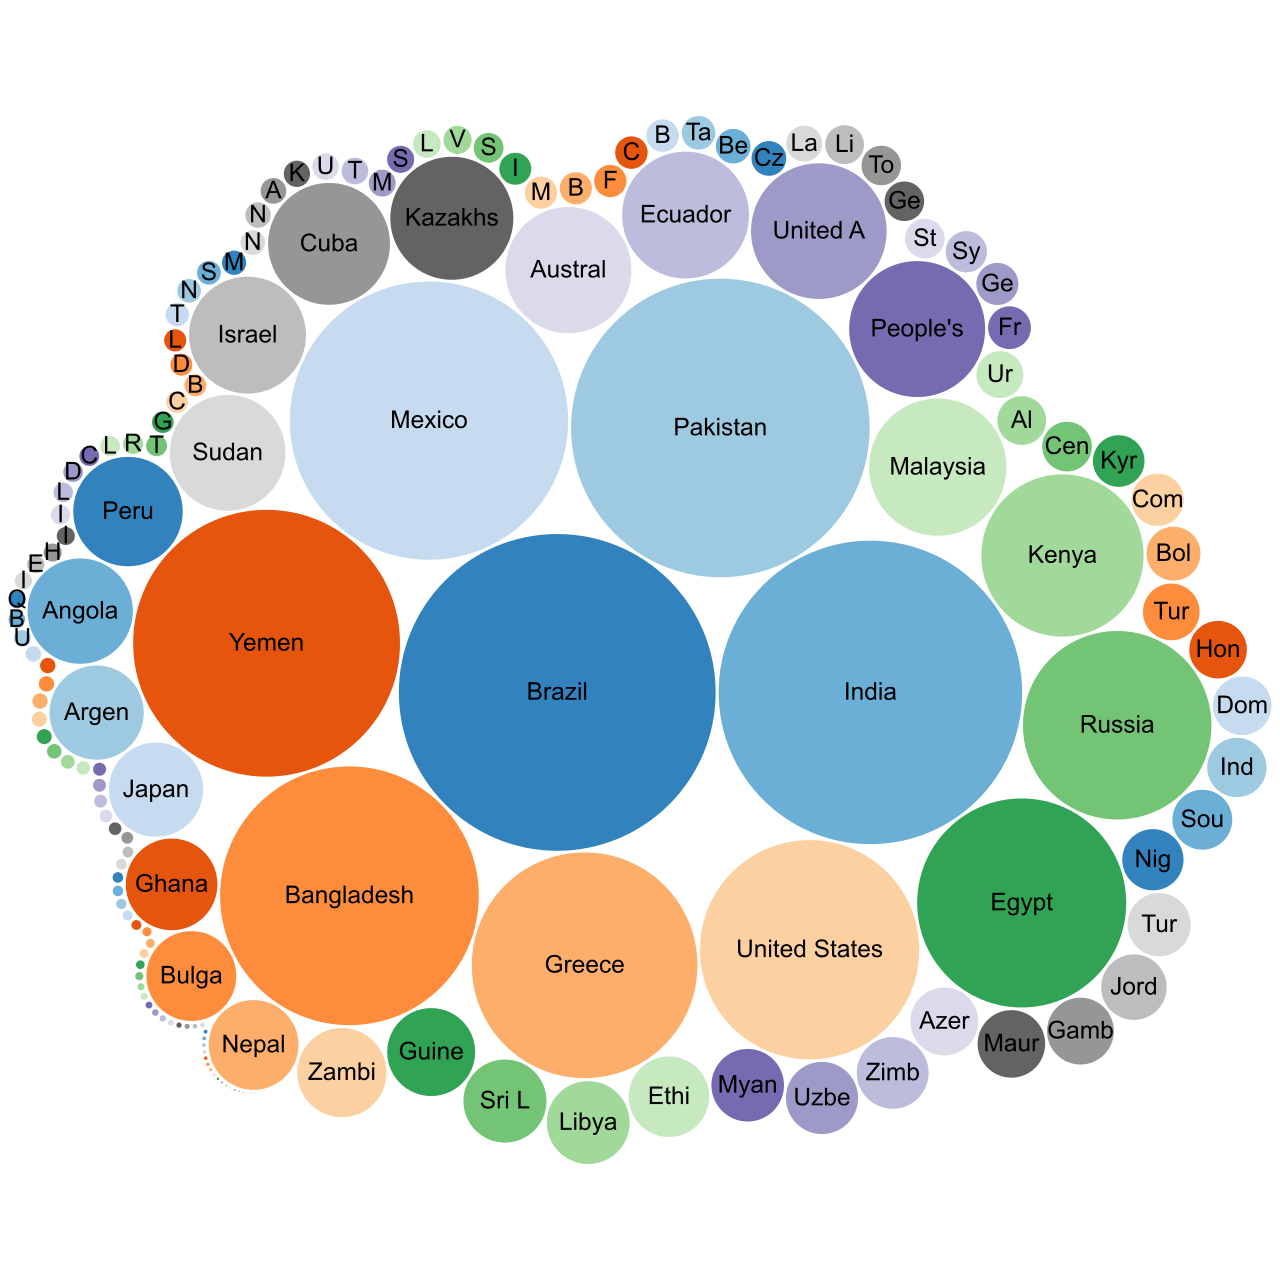
\includegraphics[width=0.9\linewidth]{./chapter/human_settlement/AnnaBubbleHumanSettlement.jpg}
	\label{fig:human-settlement-1}
    \caption[Пузырьковая диаграмма с суммарным количеством населения в населённых пунктах, 2017.]{Пузырьковая диаграмма  по суммарному количеству населения, проживающего в <<населённых пунктах>> на 2017 год. Размер пузырька соответствует количеству населения, проживающего в <<населённых пунктах>> одной страны. Ссылка на SPARQL-запрос: \href{https://w.wiki/4dAv}{https://w.wiki/4dAv}}
\end{figure}

\begin{figure}
\centering
	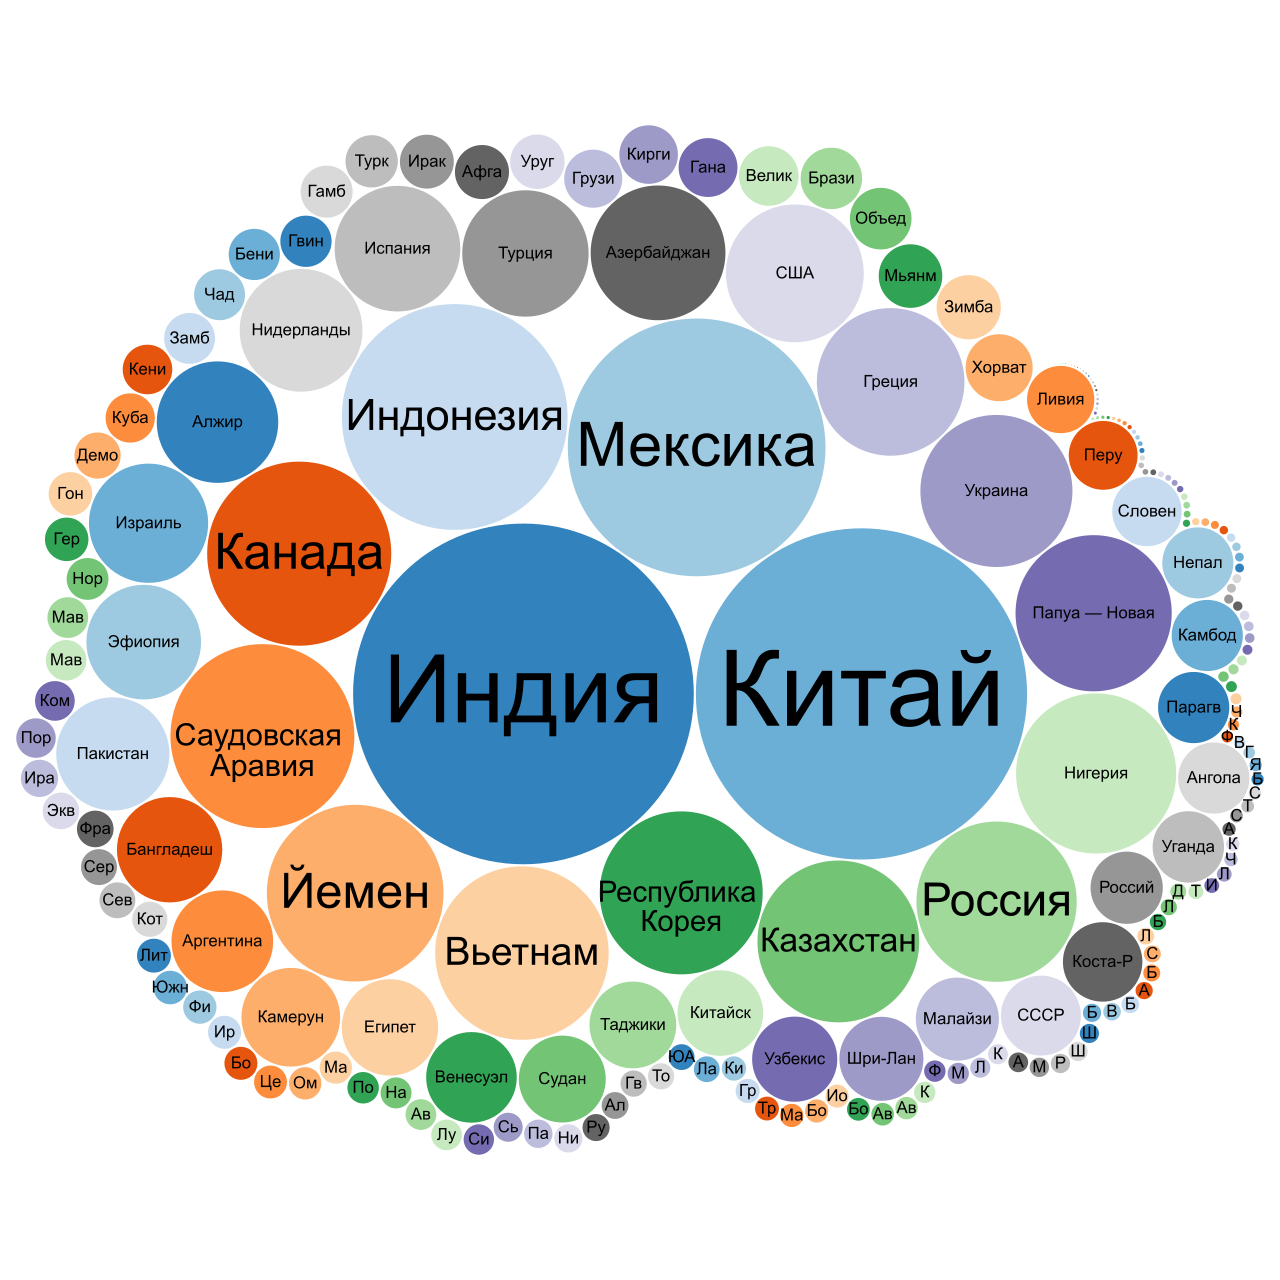
\includegraphics[width=0.9\linewidth]{./chapter/human_settlement/LeonidBubbleHumanSettlement.jpg}
	\label{fig:human-settlement-2}
	\caption[Пузырьковая диаграмма  по суммарному количеству населения в населённых пунктах, 2021.]{Пузырьковая диаграмма  по суммарному количеству населения, проживающего в <<населённых пунктах>> на 2021 год. Размер пузырька соответствует количеству населения, проживающего в <<населённых пунктах>> одной страны. Ссылка на SPARQL-запрос: \href{https://w.wiki/4dAv}{https://w.wiki/4dAv}}
\end{figure}

В 2017 году больше всего населения проживало в <<населённых пунктах>> 
\wdqName{Бразилии}{155} (\num{12} млн), 
\wdqName{Пакистана}{843} (\num{10} млн), 
\wdqName{Мексики}{96} (\num{8} млн), 
\wdqName{Йемена}{805} (\num{8} млн), 
\wdqName{Индии}{668} и 
\wdqName{Бангладеша}{902} (по \num{7} млн). 

На рис.~\ref{fig:human-settlement-2} можно увидеть список стран на 2021 год: 
\wdqName{Индия}{668} (\num{30} млн), 
\wdqName{Китай}{148} (\num{28} млн), 
\wdqName{Мексика}{96} (\num{17} млн), 
\wdqName{Индонезия}{252} (\num{13} млн), 
\wdqName{Канада}{16} (\num{9} млн) и 
\wdqName{Саудовская Аравия}{851} (\num{9} млн). 

Итак, результаты запроса~\ref{lst:human-settlement3} в 2017 и 2021 существенно разнятся. 
По этим результатам получается, что за четыре года 
в населённых пунктах Индии стало больше на 23 млн человек. 


%%%%%
\subsection{Полнота Викиданных}

Населённый пункт~--- это общее название мест с постоянными жителями\autocite{Humansettlements_Dictionary}. 
По версии редакторов Викиданных в понятие насёленный пункт входят города, сёла, деревни 
и другие\marginnote[4pt]{Полный список можно увидеть в разделе <<Cписок классов, сопутствующих ``населённому пункту'' в свойстве ``экземпляр''>> на с.~\pageref{human-settlement:tag1}.}.
Точной информации о количестве населённых пунктов в мире мы не нашли. 
Поэтому проверим полноту тех населённых пунктов, которые есть в Викиданных 
и которые использовались для решения задачи. 
В задачах выше мы использовали свойста \wdProperty{1082}{численность населения} и 
\wdProperty{17}{государство} (привязка к стране). 
Исходя из этого проверку полноты разделим на подзадачи: 
\begin{enumerate} 
  \item Проверка заполненности свойства <<численность населения>>.
  \item Проверка принадлежности к государству.
\end{enumerate}


%%%%%
\subsection{Проверка заполненности свойства <<численность населения>> }

Для такой проверки напишем \href{https://w.wiki/4FUz}{SPARQL-запрос}\sidenote{
%
В 2017 году запрос выдал \num{372997} населённых пунктов 
с незаполненным свойством <<численность населения>>. 
Тот же запрос в 2021 году выдал \num{507078} таких населённых пунктов. 
Ссылка на SPARQL-запрос: \href{https://w.wiki/4FUz}{https://w.wiki/4FUz}% 
}, 
который выведет населённые пункты 
с незаполненным свойством \href{http://www.wikidata.org/entity/P1082}{численность населения}. 
Произведя расчёты получаем, что только у 9,3\% населенных пунктов мира 
указано свойство <<численность населения>> на 2017 год. 
В 2021 получаем 11,2\% населенных пунктов мира с заполненным свойство <<численность населения>>. 
Итак, одновременно с ростом числа населённых пунктов в Викиданных 
растёт доля пунктов с заполненным свойством <<численность населения>>.


%%%%%
\subsection{Проверка принадлежности к государству}

А теперь посмотрим населённые пункты, 
у которых не указана принадлежность к какой-либо стране 
с помощью \href{https://w.wiki/4FV8}{SPARQL-запроса}\footnote{%
%
В 2017 году нашлось \num{8427} объектов, у которых не указана принадлежность к какой-либо стране. 
В 2021 году таких объектов уже больше~--- \num{27824}. 

SPARQL-запрос: \href{https://w.wiki/4FV8}{https://w.wiki/4FV8}%
}. 

Результаты запроса показывают, что число пунктов без привязки к стране растёт с годами. 
Поэтому вычисления, связанные с населёнными пунктами и странами, 
по определению будут не полными даже относительно тех пунктов, которые уже есть в Викиданных. 


%%%%%
\section{Доля населения страны, проживающего в <<населённых пунктах>>}

Построим список стран, 
упорядоченный по доли населения (в~процентах), проживающей в \href{http://www.wikidata.org/entity/Q486972}{населённых пунктах}, относительно числа всех жителей страны (листинг~\ref{lst:human-settlement6}).
%
%%%%%%%%%%%%%%%% Упражнение 2 %%%%%%%%%%%%%%%%
\begin{marginfigure}[0.0cm]
{
\includegraphics[width=0.9\linewidth]{./chapter/human_settlement/Loučovice_CoA.jpg}}
  \caption{Герб населённого пункта какой страны изображён?}%
  \label{fig:flag_question_human_settlements3}%
\end{marginfigure}
\marginnote{%
См. ответ~\ref{answer:flag_human_settlements} на с.~\pageref{answer:flag_human_settlements}.%
}

\index{SPARQL!SUM!Соотношение количества людей, проживающих в населённых пунктах, к количеству всех людей в стране}
\begin{lstlisting}[ language=SPARQL, 
                    caption={\href{https://w.wiki/4dE3}{Соотношение количества людей, проживающих в населённых пунктах, к количеству всех людей в стране}\protect\footnotemark},
                    label=lst:human-settlement6,
                    texcl 
                    ]
# An ordered list of the ratio of the number of people living in 
# "human\_settlement" to the number of inhabitants in the country.
SELECT ?country ?countryLabel ?proportionPopulation WHERE {
 SELECT ?country ?countryLabel (SUM(?population / ?pop) 
        as ?proportionPopulation) WHERE {
  ?hum wdt:P31 wd:Q486972;    # instances of human settlement  
       wdt:P17 ?country;         # has ?country 
       wdt:P1082 ?population.    # has ?population
  ?country wdt:P1082 ?pop.    # population in the country
  SERVICE wikibase:label{bd:serviceParam wikibase:language "ru,en"}
 }
 GROUP BY ?country ?countryLabel
}
ORDER BY ?proportionPopulation
\end{lstlisting}%
\footnotetext{Получено \num{158} результатов в 2017 году и \num{206} результатов в 2021 году. Ссылка на SPARQL-запрос: \href{https://w.wiki/4dE3}{https://w.wiki/4dE3}}

Столбчатая диаграмма на рис.~\ref{fig:human-settlement-3} позволяет увидеть для каждой страны 
отношение количества людей, 
проживающих в~\href{http://www.wikidata.org/entity/Q486972}{населённых пунктах}, 
к~числу жителей в~стране на 2017 год.

\begin{figure*}
    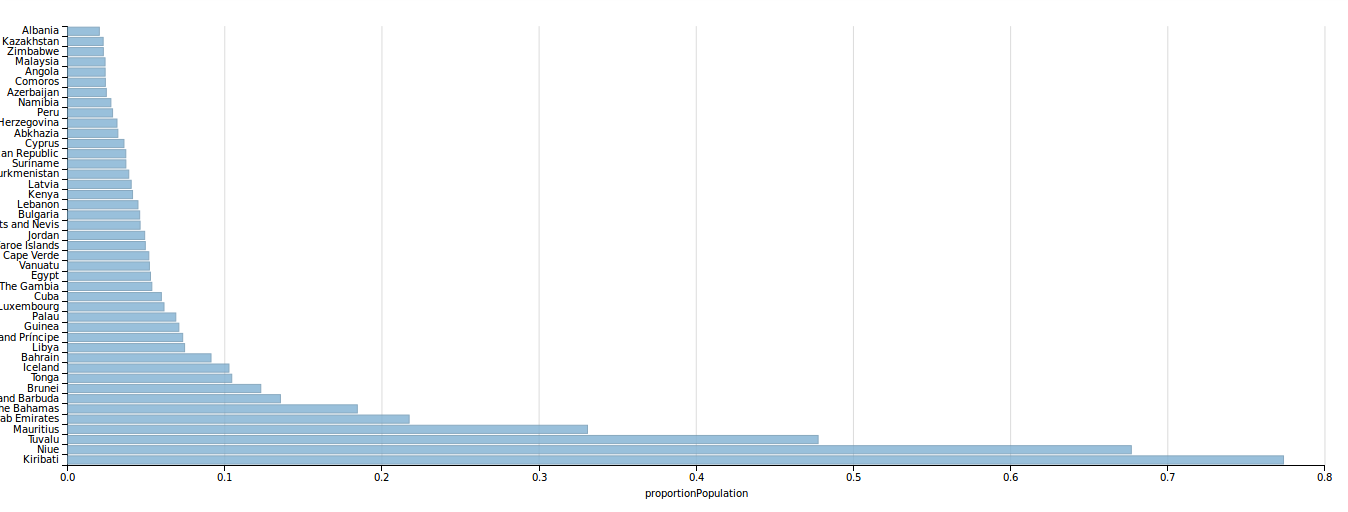
\includegraphics[width=1\linewidth]{./chapter/human_settlement/AnnaShareHumanSettlement.png}
	\label{fig:human-settlement-3}
	\caption[Диаграмма доли населения страны, 2017.]{Диаграмма доли населения страны, проживающего в <<населённых пунктах>> на 2017 год. Ссылка на SPARQL-запрос: \href{https://w.wiki/4dE3}{https://w.wiki/4dE3}}%
\end{figure*} 

\begin{figure*}
    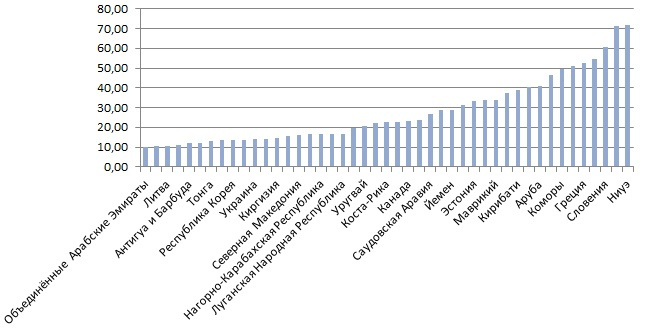
\includegraphics[width=1\linewidth]{./chapter/human_settlement/LeonidShareHumanSettlement.jpg}
	\label{fig:human-settlement-4}
	\caption[Диаграмма доли населения страны, 2021.]{Диаграмма доли населения страны, проживающего в <<населённых пунктах>> на 2021 год. Были выбраны страны с населением более 5 млн чел. SPARQL-запрос: \href{https://w.wiki/4dDx}{https://w.wiki/4dDx}}%
\end{figure*} 

По рис.~\ref{fig:human-settlement-3} видно, 
что наиболее высокий процент в 2017 году приходился на следующие страны: 
Кирибати (78\%), Ниуэ (70\%), Греция (53\%), Тувалу (48\%), Коморы (43\%), Маврикий (42\%). 
В 2021 году картина изменилась: Нигерия (93\%), Папуа~--- Новая Гвинея (71\%), 
Израиль (50\%), Греция (47\%), Азербайджан (47\%), Казахстан (37\%). 
Отметим, что в основном это маленькие островные государства. 
Вероятно, большая часть жителей этих стран сконцентрирована в~населённых пунктах.

На 2017 год в странах большой восьмёрки доля жителей 
в \href{http://www.wikidata.org/entity/Q486972}{населённых пунктах} составила: 
\href{http://www.wikidata.org/entity/Q159}{Россия} (\num{2.98}\%), 
\href{http://www.wikidata.org/entity/Q30}{США} (\num{1.76}\%), 
\href{http://www.wikidata.org/entity/Q17}{Япония} (\num{0.80}\%), 
\href{http://www.wikidata.org/entity/Q16}{Канада} (\num{0.26}\%), 
\href{http://www.wikidata.org/entity/Q142}{Франция} (\num{0.20}\%), 
\href{http://www.wikidata.org/entity/Q183}{Германия} (\num{0.24}\%), 
\href{http://www.wikidata.org/entity/Q145}{Великобритания} (\num{0.18}\%), 
\href{http://www.wikidata.org/entity/Q38}{Италия} (\num{0.07}\%). 
В 2021 году значения доли населения снизились (рис.~\ref{fig:human-settlement-4}): 
\href{http://www.wikidata.org/entity/Q159}{Россия} (0.045\%), 
\href{http://www.wikidata.org/entity/Q30}{США} (\num{0.014}\%), 
\href{http://www.wikidata.org/entity/Q17}{Япония} (\num{0.008}\%), 
\href{http://www.wikidata.org/entity/Q16}{Канада} (\num{0.23}\%), 
\href{http://www.wikidata.org/entity/Q142}{Франция} (\num{0.005}\%), 
\href{http://www.wikidata.org/entity/Q183}{Германия} (\num{0.005}\%), 
\href{http://www.wikidata.org/entity/Q145}{Великобритания} (\num{0.014}\%), 
\href{http://www.wikidata.org/entity/Q38}{Италия} (\num{0.0005}\%). 
Отметим, что это страны промышленно развитые.


%%%%%%%%%%%%%%%% Упражнение 2 %%%%%%%%%%%%%%%%
\begin{marginfigure}[0.0cm]
{
\includegraphics[width=0.9\linewidth]{./chapter/human_settlement/POL_Otynia_COA.png}}
  \caption{Герб населённого пункта какой страны изображён?}%
  \label{fig:flag_question_human_settlements4}%
\end{marginfigure}
\marginnote{%
См. ответ~\ref{answer:flag_human_settlements} на с.~\pageref{answer:flag_human_settlements}.%
}

Полученные диаграммы подтверждают следующую гипотезу: 
высокий процент населения страны, проживающего в <<населённых пунктах>>, 
указывает на более аграрную страну. 
Из диаграмм~\ref{fig:human-settlement-3} и~\ref{fig:human-settlement-4} видно, 
что наиболее высокий процент населения, проживающего в населённых пунктах, 
приходится на островные, южные, жаркие страны, 
в которых, по-видимому, менее развита промышленность 
(маленькая территория, небольшое количество населения, удалённость от материков). 
А индустриальные страны (например, страны большой восьмёрки) имеют очень низкий процент населения страны, 
проживающего в населённых пунктах.



%%%%%
\section{Cписок классов, сопутствующих <<населённому пункту>> в~свойстве <<экземпляр>>}
\label{human-settlement:tag1}

Будем называть <<классом>> такие объекты Викиданных, 
которые связаны с каким-либо объектом Викиданных посредством свойства \wdProperty{31}{экземпляр}. 
Цель этого раздела~--- найти объекты $X$, 
для которых объект \wdqName{населённый пункт}{486972} является \emph{классом}, 
и получить другие классы объекта $X$, кроме <<населённого пункта>>. 
Эти <<другие>> классы будет называть сопутствующими <<населённому пункту>>. 
С помощью запроса~\ref{lst:human-settlement7} 
найдём объекты, сопутствующие <<населённому пункту>>. 


%%%%%%%%%%%%%%%% Упражнение 2 %%%%%%%%%%%%%%%%
\begin{marginfigure}[-1.0cm]
{
\includegraphics[width=0.9\linewidth]{./chapter/human_settlement/Coat_of_Arms_of_Azov.png}}
  \caption{Герб населённого пункта какой страны изображён?}%
  \label{fig:flag_question_human_settlements5}%
\end{marginfigure}
\marginnote{%
См. ответ~\ref{answer:flag_human_settlements} на с.~\pageref{answer:flag_human_settlements}.%
}

\marginnote[1cm]{Получено 610 результатов в 2017 году и \num{1245} результатов в 2021 году. SPARQL-запрос: \href{https://w.wiki/4dEW}{https://w.wiki/4dEW}}
\begin{lstlisting}[ language=SPARQL, 
    caption={\href{https://w.wiki/4dEW}{Cписок объектов, сопутствующих <<населённому пункту>>}},
    label=lst:human-settlement7,
    texcl 
                  ]
# List of classes accompanying the human\_settlement (instance of)
SELECT ?inst (COUNT(?hum) as ?sumHum) 
WHERE{          
  ?hum wdt:P31 wd:Q486972; # instance of human settlement
       wdt:P31 ?inst.      # other objects in instance
  SERVICE wikibase:label{bd:serviceParam wikibase:language "ru,en"}
}  
GROUP BY ?inst
\end{lstlisting}%
%\footnotetext{Получено 610 результатов в 2017 году и \num{1245} результатов в 2021 году. SPARQL-запрос: \href{https://w.wiki/4dEW}{https://w.wiki/4dEW}}

Для ускорения выполнения запроса~\ref{lst:human-settlement7} выполним два шага.
 
Во-первых, выключим из рассмотрения поселения, 
имеющие в~списке экземпляров только <<населённый пункт>>, 
поскольку других сопутствующих классов нет. 
Для этого добавим в скрипт~\ref{lst:human-settlement8} строку~\num{9} с фильтром, 
требующим, чтобы у объекта \lstinline|?hum| 
кроме \wdProperty{31}{экземпляра} \wdqName{населённый пункт}{486972} был ещё какой-либо класс.

Во-вторых, в строке \num{8} запроса~\ref{lst:human-settlement8} 
уберём такие объекты переменной \lstinline|?inst|, 
которые имеют свойство \wdqName{государство}{17}. 
Это позволит отсечь сотни типов населённых пунктов специфичных для отдельных стран, 
например, <<административно-территориальная единица России>>.

Эти преобразования позволили выполнить запрос~\ref{lst:human-settlement8} 
по всем странам мира за приемлемое время в 13 мс.

\lstset{numbers=left, firstnumber=1, frame=single}
\begin{lstlisting}[ language=SPARQL, 
    caption={\href{https://w.wiki/4ePf}{Cписок классов, сопутствующих <<населённому пункту>> в свойстве <<экземпляр>> без специализированных классов разных стран}\protect\footnotemark},
    label=lst:human-settlement8,
    texcl 
                  ]
# List of objects with the class of human settlement, without 
# country and single human settlement
SELECT ?inst ?instLabel (COUNT(?hum) as ?sumHum) 
WHERE{ 
  ?hum wdt:P31 wd:Q486972;  # instance of human settlement
       wdt:P31 ?inst.       # other objects in instance
  
  MINUS {?inst wdt:P17 []}. # without country
  FILTER(?inst != wd:Q486972 ). # without human settlement
  SERVICE wikibase:label{bd:serviceParam wikibase:language "ru,en"}
}  
GROUP BY ?inst ?instLabel
ORDER BY DESC (?sumHum)
\end{lstlisting}%
\footnotetext{Получено 355 записей в 2017 году и 707 записей в 2021 году. Ссылка на SPARQL-запрос: \href{https://w.wiki/4ePf}{https://w.wiki/4ePf}}

В таблице~\ref{tab:human-settlement-classes} представлены классы, 
сопутствующие <<населённому пункту>> в свойстве <<экземпляр>>, 
и сравнение количества этих классов за 2017 и 2021 годы.

\begin{table}[h]
\centering
\begin{tabular}{|l|l|l|l|l|}
\hline
\textnumero & Название класса населённого пункта & 2017 & 2021 & $\Delta$ \\ \hline
1 & \wdqName{Cело}{532}                  & \num{2844}       & \num{4853} & +\num{2009}	\\
2 & \wdqName{Муниципалитеты}{15284}      & \num{1181}       & \num{3376} & +\num{2195}	\\
3 & \wdqName{Деревни}{5084}              & \num{662}        & \num{1761} & +\num{1099}	\\ 
4 & \wdqName{Археологические памятники}{839954}	& \num{425} & \num{887}	& +\num{462}	\\ 
5 & \wdqName{Местные поселения}{3257686} & \num{425}        & \num{158}	& -\num{257}	\\ 
6 & \wdqName{Разрушенные города}{14616455} & \num{423}      & \num{388}	& -\num{40}	\\
7 & \wdqName{Города}{515}                 & \num{322}       & \num{545}	& +\num{223}	\\
8 & \wdqName{Малые города}{3957}		  & \num{277}       & \num{446}	& +\num{169}	\\ 
9 & \wdqName{Заброшенные деревни}{350895} & \num{254}       & \num{474}	& +\num{220}	\\ 
10 & \wdqName{Внутренние районы}{2983893} & \num{207}       & \num{503}	& +\num{296}	\\ \hline
\end{tabular}
\caption{Количество классов, сопутствующих <<населённому пункту>>, в~2017 и 2021 годы, их разница ($\Delta$). 
    Получены данные по всему миру. В таблице представлены первые строки ответа на запрос~\protect\ref{lst:human-settlement9}.}
\label{tab:human-settlement-classes}
\end{table}   



Запрос~\ref{lst:human-settlement8} показал, что на 2021 год на первых местах 
среди сопутствующих <<населённому пункту>> классов 
были доисторические поселения трёх типов: поселения 
\wdqName{<<латенского периода>>}{106505016}, 
\wdqName{<<бронзового века>>}{106491277} 
и поселения \wdqName{<<доисторического времени, где есть письменность>>}{106505070}. 

Попробуем сформулировать запрос так, чтобы отсечь всё множество доисторических поселений.  
Что есть общего у этих трёх объектов на Викиданных? 
Они являются экземплярами объектов, которые, в свою очередь, 
являются экземплярами объектов \wdqName{<<археологической культуры>>}{465299}, 
\wdqName{<<исторического периода>>}{11514315}, 
\wdqName{<<археологического века>>}{15401699}, 
\wdqName{<<всемирной истории>>}{200325} 
и \wdqName{<<геологического периода>>}{392928}. 
Применим такой фильтр в запросе~\ref{lst:human-settlement9} в строках 10--12, 
чтобы отсечь именно эти типы объектов.

\index{SPARQL!COUNT!Cписок классов, сопутствующих <<населённому пункту>> в свойстве <<экземпляр>>, без исторических объектов}
\index{SPARQL!FILTER!Cписок классов, сопутствующих <<населённому пункту>> в свойстве <<экземпляр>>, без исторических объектов}
\index{SPARQL!MINUS!Cписок классов, сопутствующих <<населённому пункту>> в свойстве <<экземпляр>>, без исторических объектов}
\lstset{numbers=left, firstnumber=1, frame=single}
\begin{lstlisting}[ language=SPARQL, 
                    caption={\href{https://w.wiki/4dTq}{Cписок классов, сопутствующих <<населённому пункту>> в свойстве <<экземпляр>>, без исторических объектов}\protect\footnotemark},
                    label=lst:human-settlement9,
                    texcl 
                    ]
# List of classes accompanying the human\_settlement in the property
# 'instance of' without historical objects 
SELECT ?inst ?instLabel (COUNT(?hum) as ?sumHum) WHERE{
  ?hum wdt:P31 wd:Q486972;    # instance of human settlement
       wdt:P31 ?inst. # other objects in instance of human settlement
  ?inst wdt:P31 ?test. # instance of ?inst
  ?test wdt:P31 ?typ. # instance of ?test
  MINUS {?inst wdt:P17 []}.   # without country
  # without human settlement and prehistoric settlements
  FILTER(?inst != wd:Q486972 && ?typ != wd:Q465299 
         && ?typ != wd:Q11514315 && ?typ != wd:Q15401699 
         && ?typ != wd:Q200325 && ?typ != wd:Q392928 ). 
  SERVICE wikibase:label{bd:serviceParam wikibase:language "ru,en"}
}
GROUP BY ?inst ?instLabel
ORDER BY DESC (?sumHum)
\end{lstlisting}%
\footnotetext{Получено 89 результатов. Ссылка на SPARQL-запрос: \href{https://w.wiki/4dTq}{https://w.wiki/4dTq}}

В итоге, 707 классов запроса~\ref{lst:human-settlement8} 
мы сократили в~запросе~\ref{lst:human-settlement9} 
до 89 различных классов, сопутствующих <<населённому пункту>> в свойстве <<экземпляр>>. 
В таблице~\ref{tab:human-settlement-classes} представлены первые 10 наиболее частотных классов из 89. 


\newpage

%%%%%
\section{Отечественные учёные на селе и в городе}

Подсчитаем и сравним число отечественных учёных, родившихся в сельских и городских типах населённых пунктов. 
Решим эту задачу в пять шагов:
\begin{enumerate}
  \item Выявим список сельских и список городских типов поселений именно в России.
  \item Определим основные научные направления, представленные в~Викиданных.
  \item Выявим способ определения отечественных учёных.
  \item Сделаем такую диаграмму, на которой разным цветом будут указаны разные научные направления (математики, физики, химики и так далее) для учёных, родившихся в \emph{сельских поселениях}.
  \item Сделаем аналогичную диаграмму, но уже по \emph{городским поселениям} и сравним результаты.
\end{enumerate}


%%%%%
\subsection{Список сельских и список городских типов поселений в~России}

Выведем список типов поселений и их количество для объектов, 
имеющих свойство \wdProperty{1082}{<<численность населения>>} 
и принадлежащих \wdqName{России}{159} (листинг запроса~\ref{lst:human-settlement-noname-count}). 

\marginnote[64pt]{%
%
Задача. Используя команду FILTER~NOT~EXISTS, 
измените запрос~\ref{lst:human-settlement-noname-count} так, чтобы получить число классов 
с пустым полем <<численность населения>>. 

См. пример использования этой команды в запросе~\ref{lst:anime_no_pub_date} 
на с.~\pageref{lst:anime_no_pub_date}.%
%
}
\index{SPARQL!COUNT!Список классов поселений и их количество для объектов в России, имеющих свойство <<численность населения>>}
\begin{lstlisting}[ language=SPARQL, 
                    caption={\href{https://w.wiki/4zPi}{Список классов поселений и их количество для объектов, имеющих свойство <<численность населения>> в России}\protect\footnotemark},
                    label=lst:human-settlement-noname-count,
                    texcl 
                    ]
# List of instances of settlement with population in Russia
SELECT ?class ?classLabel (COUNT(?class) AS ?count) WHERE {
  SELECT ?class ?classLabel WHERE {
    [] wdt:P31 ?class; # noname instance of class
         wdt:P17 wd:Q159;  # in Russia
         wdt:P1082 [].     # has population
    FILTER(?class != wd:Q486972).# skip settlement itself
    SERVICE wikibase:label{bd:serviceParam wikibase:language "ru"}
  }
}
GROUP BY ?class ?classLabel
ORDER BY DESC (?count)
\end{lstlisting}%
\footnotetext{Получили 229 разных классов поселений в 2022 году. Ссылка на SPARQL-запрос: \href{https://w.wiki/4zPi}{https://w.wiki/4zPi}}

Основные классы поселений, полученные с помощью запроса~\ref{lst:human-settlement-noname-count}, 
представлены в таблице~\ref{tab:human-settlement1}. 

Обратите внимание на безымянные переменные (\lstinline|[]|) 
в строках 4~и~6 запроса~\ref{lst:human-settlement-noname-count}. 
Эта безымянность связана с тем, что 
важен факт указания численности населения, но не количество людей в них (строка~6),  
нам не нужны названия сёл и деревень (строка~4).  

Наличие строки шесть в~запросе~\ref{lst:human-settlement-noname-count} 
(\lstinline|wdt:P1082 []|) 
существенно уменьшает числа в таблице~\ref{tab:human-settlement1} 
в~столбце <<Количество>>. 
Это связано с тем, что у многих населённых пунктов 
не заполнено поле <<численность населения>>. 



\begin{table}[h]
\centering
\begin{tabular}{|r|l|c|c|}
\hline
\textnumero & Название класса & \specialcell{Количество} & Население \\ \hline
1 &\specialcell{сельское поселение\\в России (\wdq{634099})}& \num{18103} & \num{34} млн \\
2 & \wdqName{деревня}{5084}   & \num{15517}   & \num{1,8} млн\\
3 & \wdqName{село}{532}	      & \num{10204}   & \num{10,9} млн\\ 
4 & \wdqName{посёлок}{2514025} & \num{4536}   & \num{3,4} млн\\ 
7 & \wdqName{хутор}{2023000}  & \num{1782}    & \num{0,52} млн\\ 
\rowcolor{LightCyan} 
8 &\specialcell{городское поселение\\в России (\wdq{2661988})}& \num{1502} & \num{20.0} млн \\
\rowcolor{LightCyan} 
9 & \wdqName{город}{7930989}  & \num{1170}    & \num{103.6} млн\\ 
11 & \wdqName{рабочий посёлок}{20019082} & \num{583} & \num{3,7} млн\\ 
13 & \wdqName{станица}{748331} & \num{255}    & \num{1,5} млн \\
\rowcolor{LightCyan} 
20 &\specialcell{город с населением более\\\num{100000} человек (\wdq{1549591})}& \num{107} & \num{58} млн \\
\rowcolor{LightCyan} 
55 & \wdqName{город-миллионер}{1637706} & \num{14}    & \num{32.1} млн \\ \hline
\end{tabular}
\caption{Таблица классов и количество их упоминаний среди объектов, имеющих свойство <<численность населения>> в России. 
    В таблице представлены такие первые 11 строк ответа на запрос~\protect\ref{lst:human-settlement-noname-count}, 
    которые можно отнести к сельским или городским населённым пунктам. 
    Число в столбце <<\textnumero>> указывает номер строки с классом поселения 
    в списке из 229 ответов на запрос~\protect\ref{lst:human-settlement-noname-count}, 
    упорядоченных по их количству.}
\label{tab:human-settlement1}
\end{table}

Объект Викиданных \wdqName{населённый пункт}{486972} 
может быть указан в качестве класса (свойство \wdProperty{31}{экземпляр}) 
как у сельских, так и у городских поселений. 
Поэтому он нам не поможет в различении этих типов поселений 
и мы его пропускаем с помощью строки~7 запроса~\ref{lst:human-settlement-noname-count}.

Выберем из таблицы~\ref{tab:human-settlement1} строки без подсветки, 
то есть классы под номерами 1, 2, 3, 4, 7, 11 и 13. 
В~дальнейшем комбинацию этих классов будем называть \emph{сельские поселения}. 
Подсчитаем, сколько всего людей живёт в таких поселениях в России\footnote{Получили \num{55,6} млн человек. 
Ссылка на SPARQL-запрос: \url{https://w.wiki/4$D6}%
}. 

\newpage
Суммарное число жителей по каждому из классов \emph{сельских поселений} 
вычислим с помощью запроса~\ref{lst:human-settlement-village-count}. 
Полученные числа представлены в таблице~\ref{tab:human-settlement1} в столбце <<Население>>. 
Если запрос~\ref{lst:human-settlement-village-count} выполняется слишком долго, 
вы можете закомментировать или удалить часть классов в строках 3--4 
и тем самым упростить и ускорить обработку запроса. 

\index{SPARQL!VALUES!Классы сельских поселений}
\begin{lstlisting}[ language=SPARQL, 
                    caption={\href{https://w.wiki/4$8w}{Список классов сельских поселений в России и суммарное число жителей по каждому классу}\protect\footnotemark},
                    label=lst:human-settlement-village-count,
                    texcl 
                    ]
# Number of population living in villages
SELECT ?village ?villageLabel (SUM(?population) AS ?count) WHERE {  
  VALUES ?village {wd:Q634099 wd:Q5084 wd:Q532 wd:Q2514025 
                   wd:Q2023000 wd:Q20019082 wd:Q748331}
  [] wdt:P17 wd:Q159;  # settlement in the Russia
     wdt:P1082 ?population; # has ?population
     wdt:P31 ?village. # instance of ?village (see the list)
 SERVICE wikibase:label{bd:serviceParam wikibase:language "ru"}
}
GROUP BY ?village ?villageLabel
\end{lstlisting}%
\footnotetext{Число жителей в сельских поселениях России в 2022 году представлено в таблицы~\ref{tab:human-settlement1} в столбце <<Население>>. Ссылка на SPARQL-запрос: \url{https://w.wiki/4$8w}}



А набор классов под номерами 8, 9, 20 и 55 в таблице~\ref{tab:human-settlement1} 
назовём \emph{городскими поселениями}. 
Подсчитаем суммарное число жителей в~городских поселениях России 
с помощью запроса~\ref{lst:human-settlement-count-total-city}. 


\begin{lstlisting}[ language=SPARQL, 
                    caption={\href{https://w.wiki/4$D9}{Суммарное число жителей в~городских поселениях России}\protect\footnotemark},
                    label=lst:human-settlement-count-total-city,
                    texcl 
                    ]
# Number of population living in cities
SELECT (SUM(?population) AS ?count) WHERE {  
  SELECT DISTINCT ?city ?population WHERE {  
    VALUES ?city_list {wd:Q7930989 wd:Q2661988 wd:Q1549591 wd:Q1637706}
    ?city wdt:P17 wd:Q159;       # settlement in Russia
          wdt:P1082 ?population; # has ?population
          wdt:P31 ?city_list.    # instance of ?city
  }
}
\end{lstlisting}%
\footnotetext{Число жителей в городских поселениях России в 2022 году составило \num{116,1} млн человек. 
Ссылка на SPARQL-запрос: \url{https://w.wiki/4$D9}}

Суммарное число жителей по каждому из классов \emph{городских поселений} 
вычисляется аналогично запросу~\ref{lst:human-settlement-village-count}. 
Полученные числа представлены в таблице~\ref{tab:human-settlement1} в столбце <<Население>>. 

Таким образом, получили, что \num{55.6} млн человек живёт в сельских поселениях и \num{116.1} млн человек~--- в городских. 
Общее число составило \num{171.7} млн человек. 
при этом по оценке Росстата в России было 145 млн человек на 2022 год. 
Получили на 27 млн человек больше, и это с учётом того, что Викиданные достаточно неполные. 

На наш взгляд, проблема подсчётов заключается в том, 
что большие города включают в себя множество небольших городков и жители этих городков считаются дважды. 
Команда \lstinline|DISTINCT|%
%
%
\TFfootnote{Команда \lstinline|DISTINCT| в~строке~3 запроса~\ref{lst:human-settlement-count-total-city} 
нужна для учёта случаев, когда одному населённому пункту \lstinline|?city| 
соответствует несколько значений списка \lstinline|?city_list| в~строке~7. 
То есть населённый пункт может одновременно быть \wdProperty{31}{экземпляром} 
\wdqName{города}{7930989} и \wdqName{города-миллионера}{1637706}. 

Команда \lstinline|DISTINCT| во внутреннем цикле \lstinline|SELECT| (строки~3--8) 
позволяет получить эти города (\lstinline|?city|) без дублирования. 
Если убрать слово \lstinline|DISTINCT| из запроса, 
то численность населения вырастет со \num{116.1} млн до \num{187.2} млн человек. 

Отметим, что если сложить численность разных типов городов в таблице~\ref{tab:human-settlement1}, 
то получим $20 + 103.6 + 58 + 32.1 = 213.7$. 
Очевидно, что списки разных типов городских поселений пересекаются, поэтому получилось такое большое число.%
} 
%
%
в запросе~\ref{lst:human-settlement-count-total-city} 
эту проблему не решает, поскольку это разные объекты. 
Один из вариантов решения заключается в том, 
чтобы дополнительно проверять населённые пункты~---  
не входят ли они в более крупные населённые пункты, 
и если входят, то не считать их население повторно. 



%%%%%
\subsection{Профессии, представленные в Викиданных}

Получим список профессий и количество работников, 
имеющих российское гражданство. 
Этим запросом (листинг~\ref{lst:human-settlement13}) 
мы ищем такие объекты Викиданных, 
у которых есть свойство \wdProperty{27}{гражданство} 
и значением этого свойства является объект \wdqName{Россия}{159}. 
Очевидно, что объект, имеющий свойство <<гражданство>>, будет человеком 
или в терминологии вики-проектов~--- персоной. 


\index{SPARQL!COUNT!Список профессий или должностей граждан России}
\lstset{numbers=left, firstnumber=1, frame=single}
\begin{lstlisting}[ language=SPARQL, 
                    caption={\href{https://w.wiki/4daC}{Список профессий или должностей граждан России}\protect\footnotemark},
                    label=lst:human-settlement13,
                    texcl 
                    ]
# List of occupation or job citizens of Russia 
SELECT DISTINCT ?job ?jobLabel (COUNT(?hum) AS ?count) WHERE {
  ?hum wdt:P27 wd:Q159; # citizen of Russia 
       wdt:P106 ?job. # has occupation or job
  SERVICE wikibase:label{bd:serviceParam wikibase:language "ru,en"}
}
GROUP BY ?job ?jobLabel
ORDER BY ?count
\end{lstlisting}%
\footnotetext{Получено 2023 профессии на 2022 год. Ссылка на SPARQL-запрос: \href{https://w.wiki/4daC}{https://w.wiki/4daC}}

В таблице~\ref{tab:human-settlement3} представлены такие профессии  
из~результата запроса~\ref{lst:human-settlement13}, 
которые могут соответствовать каким-либо научными направлениям.

\begin{table}[h]
\centering
\begin{tabular}{|r|l|c|}
\hline
\textnumero & Профессия (объект) & Число людей \\ \hline
1 & \wdqName{физик}{169470}     & \num{991} \\
2 & \wdqName{историк}{201788}   & \num{913} \\
3 & \wdqName{экономист}{188094}	& \num{880} \\ 
4 & \wdqName{математик}{170790}	& \num{857} \\ 
5 & \wdqName{инженер}{81096}	& \num{558} \\ 
7 & \wdqName{химик}{593644}		& \num{439} \\ 
8 & \wdqName{врач}{39631}		& \num{342} \\ 
9 & \wdqName{юрист}{185351}		& \num{330} \\ 
10 & \wdqName{биолог}{864503}	& \num{222} \\ \hline
\end{tabular}
\caption{Таблица научных направлений и их количество упоминаний среди людей с Росиийским гражданством}
\label{tab:human-settlement3}
\end{table}

%%%%%
\subsection{Найти учёных среди людей}

Есть два способа получения списка учёных. 
Первый~--- у большинства учёных в Викиданных заполнено свойства \wdProperty{512}{научная степень}. 
Запросим в Викиданных россиян, имеющих такое свойство (листинг~\ref{lst:human-settlement14}), 
и получим список отечественных учёных. 

На полях: Зачем нужна команда \lstinline|DISTINCT| в~строке~??? запроса~\ref{lst:human-settlement14}? 
Почему без этой команды число учёных не~изменится, а~число записей с~ответами увеличится?

\index{SPARQL!COUNT!Количество людей из России с учёной степенью}
\begin{lstlisting}[ language=SPARQL, 
                    caption={\href{https://w.wiki/4deJ}{Количество людей из России с учёной степенью}\protect\footnotemark},
                    label=lst:human-settlement14,
                    texcl 
                    ]
# Count of peoples in Russian with academic degree
SELECT (COUNT(DISTINCT ?hum) AS ?human_count) WHERE {
  # Russian Empire, Soviet Union and Russia
  VALUES ?ruCountries {wd:Q34266 wd:Q15180 wd:Q159}
  ?hum wdt:P512 ?academic_degree;  # has academic degree 
       wdt:P27 ?ruCountries. # lives (lived) in Russian countries
  SERVICE wikibase:label{bd:serviceParam wikibase:language "ru,en"}
}
\end{lstlisting}%
\footnotetext{Получено 24297 человек. Ссылка на SPARQL-запрос: \href{https://w.wiki/4deJ}{https://w.wiki/4deJ}}

Второй по наличию свойства \wdProperty{463}{участник организации} нескольких академий: \wdqName{academy of sciences}{414147}, \wdqName{learned society}{955824}, \wdqName{scientific society}{74801}, \wdqName{academy}{162633}, \wdqName{research institute}{31855}, \wdqName{educational institution}{2385804 }. Выведем список людей имеющих такое свойство (листинг~\protect\ref{lst:human-settlement15}). 

\index{SPARQL!COUNT!Количество людей из академий в России}
\begin{lstlisting}[ language=SPARQL, 
                    caption={\href{https://w.wiki/4deV}{Количество людей из академий в России}\protect\footnotemark},
                    label=lst:human-settlement15,
                    texcl 
                    ]
# Count of peoples in Russian in academy
SELECT (COUNT(DISTINCT ?hum) AS ?human_count) WHERE {
  VALUES ?ruCountries {wd:Q34266 wd:Q15180 wd:Q159}
  VALUES ?class_academy {wd:Q414147 wd:Q955824 wd:Q74801 wd:Q162633 
                      wd:Q31855 wd:Q2385804 wd:Q83172}
  ?hum wdt:P463 ?academy;  # has academic degree 
       wdt:P27 ?ruCountries. # lives (lived) in countries
  # academy is an element of the class academy
  ?academy wdt:P31 ?class_academy. 
  SERVICE wikibase:label{bd:serviceParam wikibase:language "ru,en"}
}
\end{lstlisting}%
\footnotetext{Получено 4170 человек. Ссылка на SPARQL-запрос: \href{https://w.wiki/4deV}{https://w.wiki/4deV}}

Первый способ дает больше людей, что позволить увидеть более подробную картину на диаграммах ниже. Будем его использовать для построения диаграмм ниже.

%%%%%
\subsection{Построение диаграммы на которой разным цветом будут указаны разные научные направления для учёных родившихся в сельских поселениях}

Используя вышеописанные шаги, получаем запрос~\protect\ref{lst:human-settlement16}.

\index{SPARQL!COUNT!Диаграмма количества ученых по родам деятельности родившихся в сельских поселениях}
\index{SPARQL!FILTER!Диаграмма количества ученых по родам деятельности родившихся в сельских поселениях}
\index{SPARQL!FLOOR!Диаграмма количества ученых по родам деятельности родившихся в сельских поселениях}
\index{SPARQL!YEAR!Диаграмма количества ученых по родам деятельности родившихся в сельских поселениях}
\index{SPARQL!STR!Диаграмма количества ученых по родам деятельности родившихся в сельских поселениях}
\index{SPARQL!BIND!Диаграмма количества ученых по родам деятельности родившихся в сельских поселениях}
\index{SPARQL!GROUP BY!Диаграмма количества ученых по родам деятельности родившихся в сельских поселениях}
\index{График!BarChart!Диаграмма количества ученых по родам деятельности родившихся в сельских поселениях}

\begin{lstlisting}[ language=SPARQL, 
                    caption={\href{https://w.wiki/xxxx}{Диаграмма количества ученых по родам деятельности родившихся в сельских поселениях}\protect\footnotemark},
                    label=lst:human-settlement16,
                    texcl 
                    ]
# defaultView:BarChart
# Diagram of the number of scientists by occupation in rural settlements

\end{lstlisting}%
\footnotetext{Ссылка на SPARQL-запрос: \href{https://w.wiki/xxxx}{https://w.wiki/xxxx}}

Диаграмма~\ref{fig:human-settlement-5} показывает количество учёных по родам деятельности, 
родившихся в сельских поселениях.

\begin{figure*}
    \setlength{\fboxsep}{0pt}%
    \setlength{\fboxrule}{1pt}%
    \fcolorbox{gray}{gray}{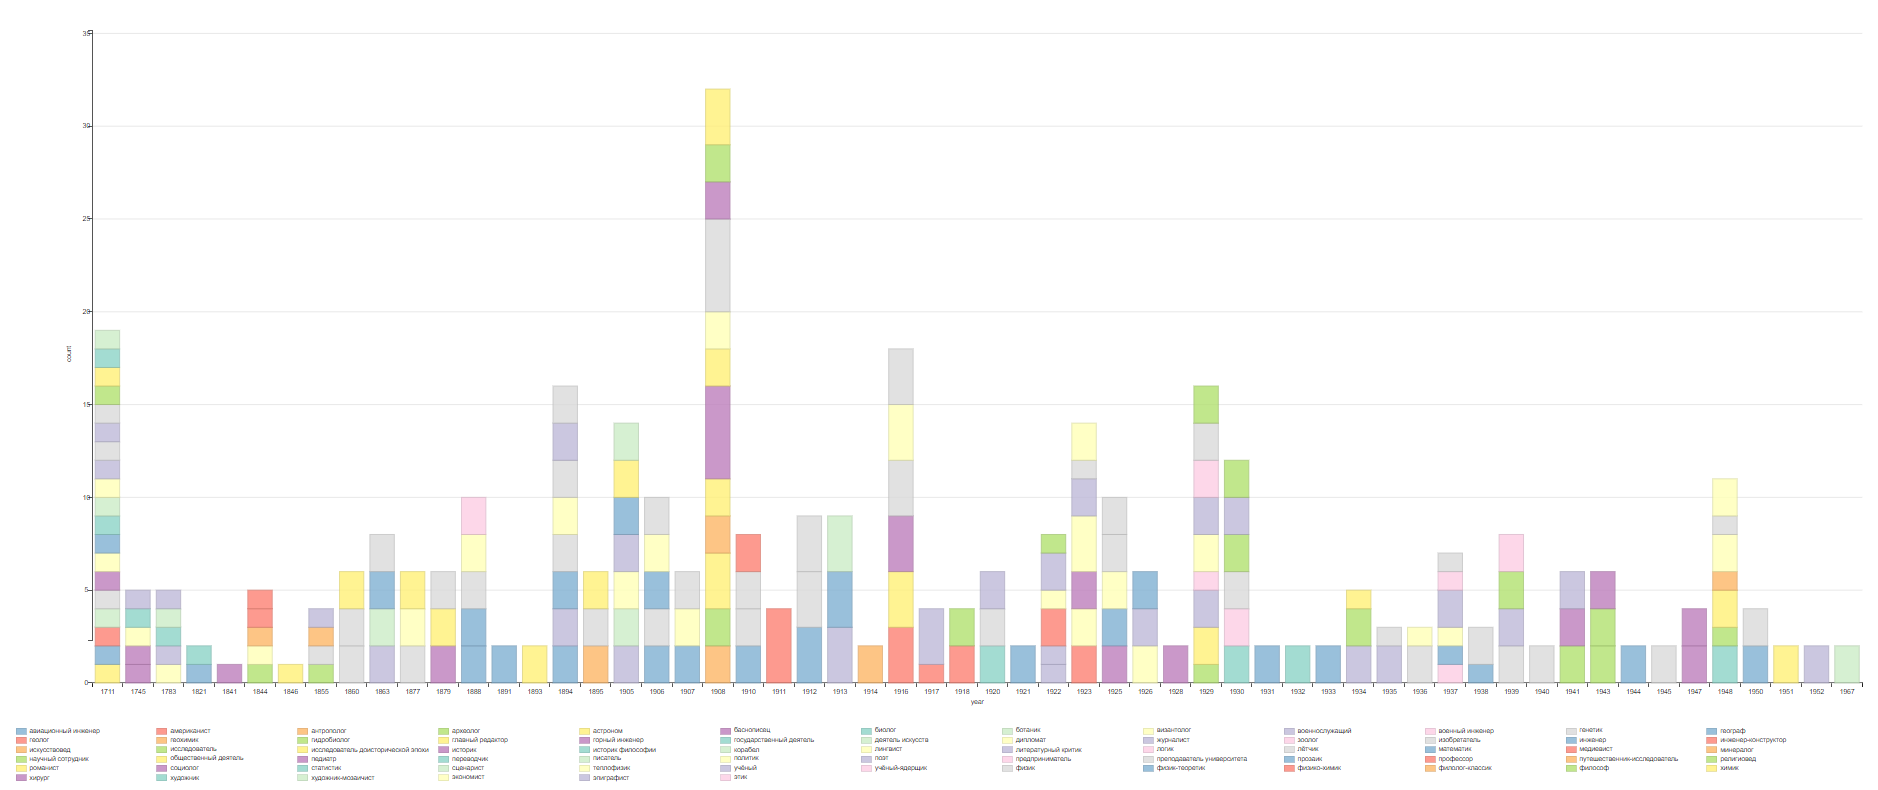
\includegraphics[width=1\linewidth]{./chapter/human_settlement/RussianScientistBornVillage.png}}
	\label{fig:human-settlement-5}
	\caption[Диаграмма количества ученых по родам деятельности родившихся в сельских поселениях.]{Диаграмма количества ученых по родам деятельности родившихся в сельских поселениях. Ссылка на SPARQL-запрос: \href{https://w.wiki/xxxx}{https://w.wiki/xxxx}.}%
\end{figure*} 

%%%%%
\subsection{Построение диаграммы для учёных родившихся в городских поселениях и сравнение диаграмм}

Используя вышеописанные шаги, получаем такой запрос~\ref{lst:human-settlement17}.

\index{SPARQL!COUNT!Диаграмма количества ученых по родам деятельности родившихся в городских поселениях}
\index{SPARQL!FILTER!Диаграмма количества ученых по родам деятельности родившихся в городских поселениях}
\index{SPARQL!FLOOR!Диаграмма количества ученых по родам деятельности родившихся в городских поселениях}
\index{SPARQL!YEAR!Диаграмма количества ученых по родам деятельности родившихся в городских поселениях}
\index{SPARQL!STR!Диаграмма количества ученых по родам деятельности родившихся в городских поселениях}
\index{SPARQL!BIND!Диаграмма количества ученых по родам деятельности родившихся в городских поселениях}
\index{SPARQL!GROUP BY!Диаграмма количества ученых по родам деятельности родившихся в городских поселениях}
\index{График!BarChart!Диаграмма количества ученых по родам деятельности родившихся в городских поселениях}

\begin{lstlisting}[ language=SPARQL, 
                    caption={\href{https://w.wiki/xxxx}{Диаграмма количества ученых по родам деятельности родившихся в городских поселениях}\protect\footnotemark},
                    label=lst:human-settlement17,
                    texcl 
                    ]
# defaultView:BarChart
# Diagram of the number of scientists by occupation in town settlements

\end{lstlisting}%
\footnotetext{Ссылка на SPARQL-запрос: \href{https://w.wiki/xxxx}{https://w.wiki/xxxx}}

Диаграмма~\ref{fig:human-settlement-6} показывает количество учёных по родам деятельности, родившихся в городских полесениях.

\begin{figure*}
    \setlength{\fboxsep}{0pt}%
    \setlength{\fboxrule}{1pt}%
    \fcolorbox{gray}{gray}{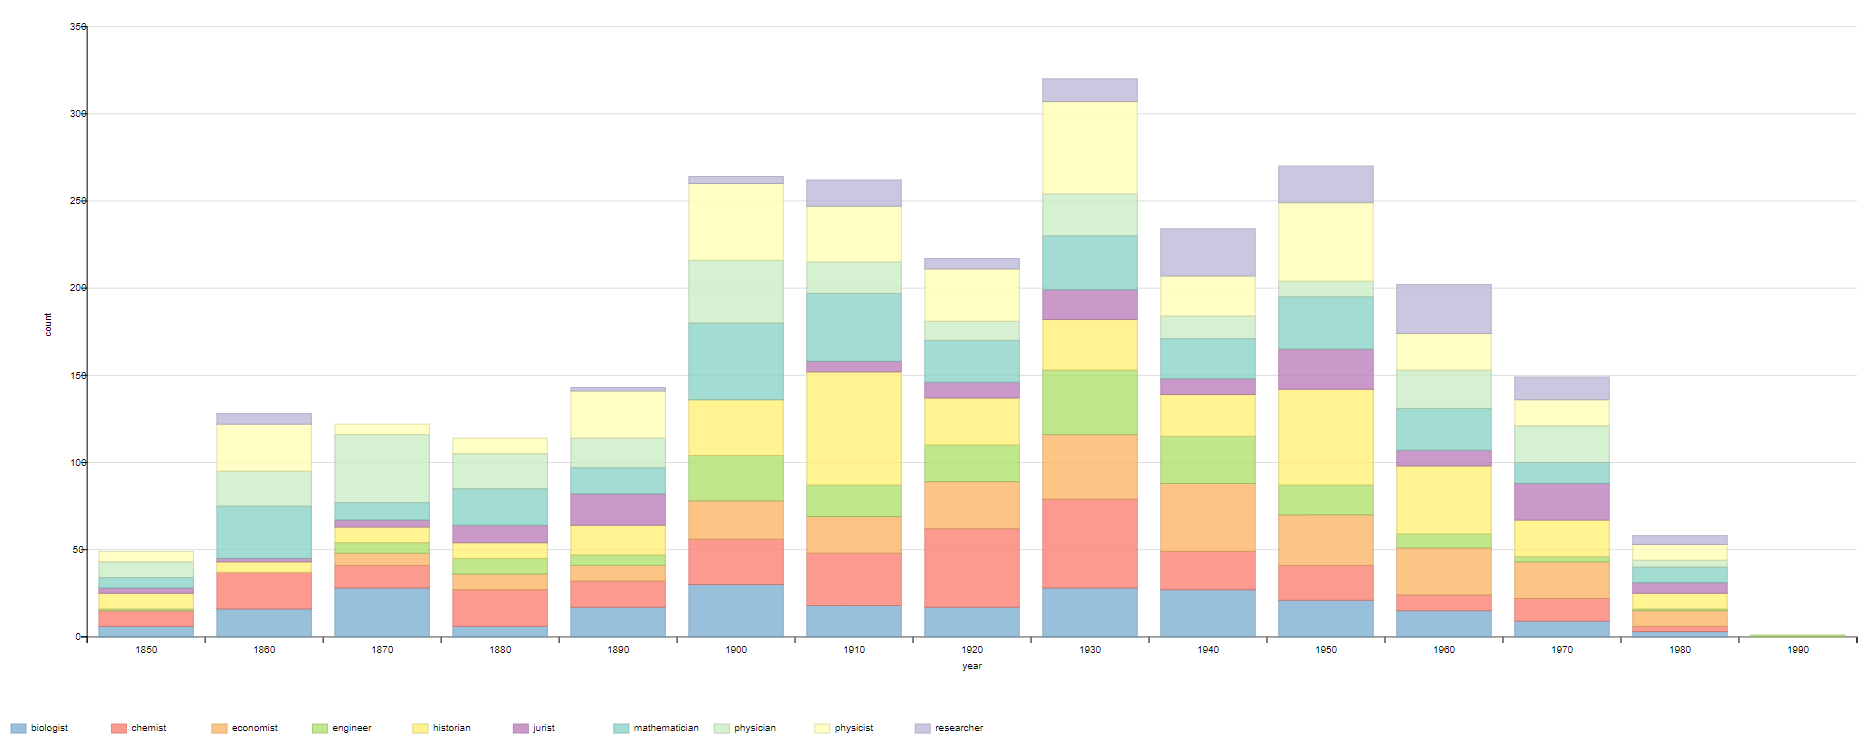
\includegraphics[width=1\linewidth]{./chapter/human_settlement/RussianScientistBornTown.png}}
	\label{fig:human-settlement-6}
	\caption[Диаграмма количества ученых по родам деятельности родившихся в городских поселениях.]{Диаграмма количества ученых по родам деятельности родившихся в городских поселениях. Ссылка на SPARQL-запрос: \href{https://w.wiki/xxxx}{https://w.wiki/xxxx}}%
\end{figure*} 

Сравнив диаграммы, видно что ученных в городских поселениях больше примерно в 3 раза, чем в сельских поселениях. Выше мы считали количество населения с этих группах, разница в населении достигает почти в 4 раза. Следовательно можно сказать, что не важно где ты родился. 
